%% labapi software metapaper for the Journal of Open Research Software.
%% Built on the official JORS LaTeX template (version 0.2, class jors.cls).
%%
%% Build from this directory (CI: .github/workflows/draft-pdf.yml, job jors):
%%   rsvg-convert -f pdf -o ../figures/object-model.pdf ../figures/object-model.svg
%%   pdflatex jors && bibtex jors && pdflatex jors && pdflatex jors
%%
%% Open items are marked "TODO" in comments.

\documentclass{jors}

% JORS uses numbered (Vancouver) citations; unsrtnat numbers references in
% order of first citation.
\usepackage[numbers,sort&compress]{natbib}
\usepackage{graphicx}

\pagestyle{fancy}
\definecolor{mygray}{gray}{0.6}
\renewcommand\headrule{}
\rhead{\textcolor{gray}{labapi: JORS software metapaper}}

\begin{document}

\rule{\textwidth}{1pt}

\section*{(1) Overview}

\vspace{0.5cm}

\section*{Title}

labapi: a Python object model for the LabArchives electronic lab notebook

\section*{Paper Authors}

1. Li, Christoph; \\
2. Lawrimore, Josh; \\
3. Moraczewski, Dustin; \\
4. Thomas, Adam G.

\section*{Paper Author Roles and Affiliations}

1. Software; Writing -- original draft. Data Science and Sharing Team,
National Institute of Mental Health, National Institutes of Health,
Bethesda, MD, USA. ORCID 0009-0009-4624-2578. Corresponding author:
christoph.li@nih.gov \\
2. Conceptualization; Software; Writing -- review \& editing. Clinical
Monitoring Research Program Directorate, Frederick National Laboratory for
Cancer Research, Frederick, MD, USA. ORCID 0000-0003-2301-9073 \\
3. Supervision; Writing -- review \& editing. Data Science and Sharing Team,
National Institute of Mental Health, National Institutes of Health,
Bethesda, MD, USA. ORCID 0000-0002-0422-3135 \\
4. Supervision; Writing -- review \& editing. Data Science and Sharing Team,
National Institute of Mental Health, National Institutes of Health,
Bethesda, MD, USA. ORCID 0000-0002-2850-1419

\section*{Abstract}

Researchers often copy the outputs of analysis pipelines into their
electronic lab notebook by hand.
labapi is a Python library that lets pipelines read from and write to the
LabArchives notebook directly. Code names a page by the folder path a
researcher sees in the web interface, such as Partly Cloudy QC/sub-01, and
labapi finds or creates the matching page through the API. The library is
released under the MIT licence, archived on Zenodo and installable from
PyPI. To use it, a laboratory needs API credentials, which LabArchives
issues through the institution.

\section*{Keywords}

electronic lab notebook; LabArchives; research data management;
laboratory record-keeping; reproducibility; Python

\section*{Introduction}

Once an output is added to a LabArchives page, it sits beside the notes and
revision history that document the experiment \citep{labarchives}. Getting
it there usually means opening the web interface after each pipeline run and
uploading by hand. LabArchives is a widely used commercial electronic lab
notebook (ELN) and one of the notebooks approved for new research in the NIH
Intramural Research Program \citep{nih_eln_policy}. Its web API can automate
the upload, but it identifies pages by internal tree IDs and returns a
notebook one folder level per call \citep{labarchives_api}. Code that wants
to write to Partly Cloudy QC/sub-01 has to list the top level of the
notebook, find the folder by name, list that folder, find the page, and only
then sign and send the request that adds the entry. Each laboratory that
automates its record-keeping ends up writing this code for itself.

labapi does the lookup and the signing, and creates missing folders and
pages on request. At NIMH, two applications are built on it: muronto records
neuro-behavioural experiment outputs, and save-my-jupyter deposits Jupyter
notebook snapshots \citep{muronto,save_my_jupyter}. It is aimed at
computational researchers and research software engineers in laboratories
that use LabArchives.

Benchling, RSpace and eLabFTW each ship an official Python client for their
API \citep{benchling_sdk,rspace_client,elabapi_python}, but LabArchives has
none.
None of the public standalone LabArchives clients in
Table~\ref{tab:comparison} offers path-based access to notebooks. The
closest, labarchives-py, is a single module that signs arbitrary GET
requests and returns the raw responses. Choosing endpoints, parsing the XML
and walking the tree are left to the caller. Building those on top of it
would have meant writing the notebook model anyway, so labapi was started as
a separate client. There are also LabArchives integrations for the ReDBox
research data portal and for the Model Context Protocol, but neither offers
a general Python interface to notebooks
\citep{redbox_labarchives,labarchives_mcp}.

% TODO: re-check each row against the current state of each project and
% update the date in the caption before submission.
\begin{table}[htbp]
	\centering
	\caption{Public standalone LabArchives clients, checked 20 August 2026.}
	\label{tab:comparison}
	\small
	\begin{tabular}{lp{5.5cm}p{2.6cm}}
		\hline
		\textbf{Project} & \textbf{What it provides} & \textbf{Navigable notebook objects} \\
		\hline
		labapi & General Python client & Yes \\
		labarchives-py \citep{mcmero} & Signed generic GET-call wrapper & No \\
		labarchives-js \citep{marcellofuschi} & Login, image-entry search, attachment URLs & No \\
		labarchives-client \citep{alaninmcr} & Unmaintained; no released functionality & No \\
		\hline
	\end{tabular}
\end{table}

\section*{Implementation and architecture}

The code has four layers. At the bottom, the client signs each request with
HMAC-SHA512 and handles login. Above it, a user session holds the notebooks a
researcher can open, and the tree layer models their folders and pages. Page
content, whether rich text, headers, plain text, attachments or widgets, is
handled by the entry layer. Responses arrive as XML and are parsed with
lxml.

Each folder and page in the tree layer corresponds to one in the web
interface (Figure~\ref{fig:model}). A folder's contents are fetched with a
single \texttt{get\_tree\_level} call the first time code looks inside it.
\texttt{dir()} and \texttt{page()} return the folder or page at a path,
creating it and any missing parent folders if needed. \texttt{traverse()}
follows only paths that already exist.

\begin{figure}[htbp]
    \centering
    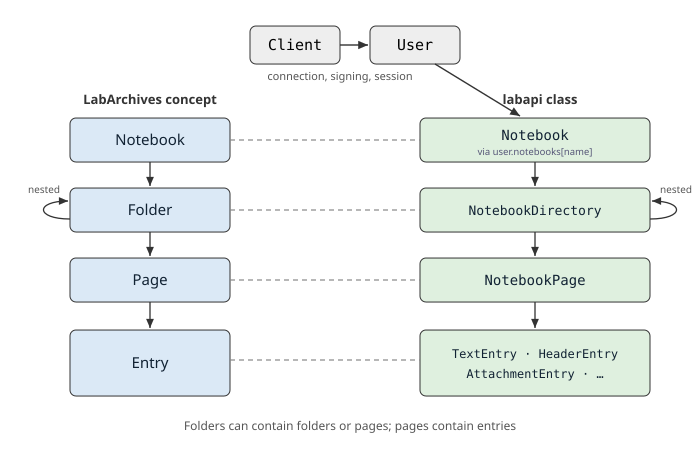
\includegraphics[width=0.64\textwidth]{../figures/object-model}
    \caption{The LabArchives notebook hierarchy and the corresponding labapi
    objects.}
    \label{fig:model}
\end{figure}

Path strings are parsed once, following Alexis King's ``parse, don't
validate'' \citep{king2019parse}, into \texttt{NotebookPath} objects that
record their segments and whether they are absolute or relative. Joining,
resolving, containment checks and traversal all work on these objects.

\texttt{create\_json\_entry()} stores JSON as an attachment that code can
read back, and adds a formatted preview for people reviewing the page in the
web interface. A library-level meta-entry that grouped the two was
considered. It would have broken the direct correspondence between labapi
objects and native LabArchives entries, and other tools would then have
needed extra bookkeeping entries to preserve the grouping. Richer metadata
schemes are left to the applications built on labapi.

API credentials are held in a \texttt{Client} object, separate from the
\texttt{User} sessions it creates. One service can hold sessions for
several researchers without handing out the credentials.

\section*{Quality control}

The unit tests cover request signing and authentication, path parsing, tree
navigation, entry handling, notebook backup and the bundled examples. They
mock the network layer and need no credentials. An integration suite runs
the same operations against a live LabArchives account and is started by
hand. On every push and pull request, GitHub Actions runs the unit tests on
Python 3.10 to 3.14, along with Ruff lint and format checks, static type
checking and a documentation build.

The repository's examples directory contains runnable workflows with sample
input data, and each example is covered by the unit tests. The JSON
synchronisation example is the quickest check that an installation works. It
uploads the two JSON files in its \texttt{sample\_data} folder to a notebook
page as JSON entries, and its download command writes them back to local
files that should match the originals.

A fuller example is a two-stage quality-control workflow for five subjects
from the public OpenNeuro dataset ds000228 \citep{ds000228}. In the
listings, \texttt{subjects} stands for the five subject identifiers, and
\texttt{compute\_qc()} and \texttt{summarize()} stand for the scientific
calculations. The first stage writes, for each subject, a group label and
the mean DVARS, a quality-control measure of how much a functional MRI scan
changes between successive time points \citep{power2012dvars}. It creates or
reuses one page per subject in an existing notebook:

{\footnotesize
\begin{verbatim}
user = labapi.Client().default_authenticate()
qc = user.notebooks["Lab QC"].dir("Partly Cloudy QC")

for subject in subjects:
    qc.page(f"sub-{subject}").entries.create_json_entry(compute_qc(subject))
\end{verbatim}
}

The second stage reads the stored values back, produces a cohort summary and
a figure, and writes both to a dashboard page:

{\footnotesize
\begin{verbatim}
notebook = user.notebooks["Lab QC"]
qc = notebook.traverse("Partly Cloudy QC")
records = [json.load(page.entries[0].content) for page in qc.children]

summary, figure_path = summarize(records)
dashboard = notebook.page("Dashboards/Cohort QC")
dashboard.entries.create_json_entry(summary)

attachment = labapi.Attachment.from_file(figure_path)
dashboard.entries.create(labapi.AttachmentEntry, attachment)
\end{verbatim}
}

The resulting LabArchives page is shown in Figure~\ref{fig:dashboard}.

\begin{figure}[htbp]
    \centering
    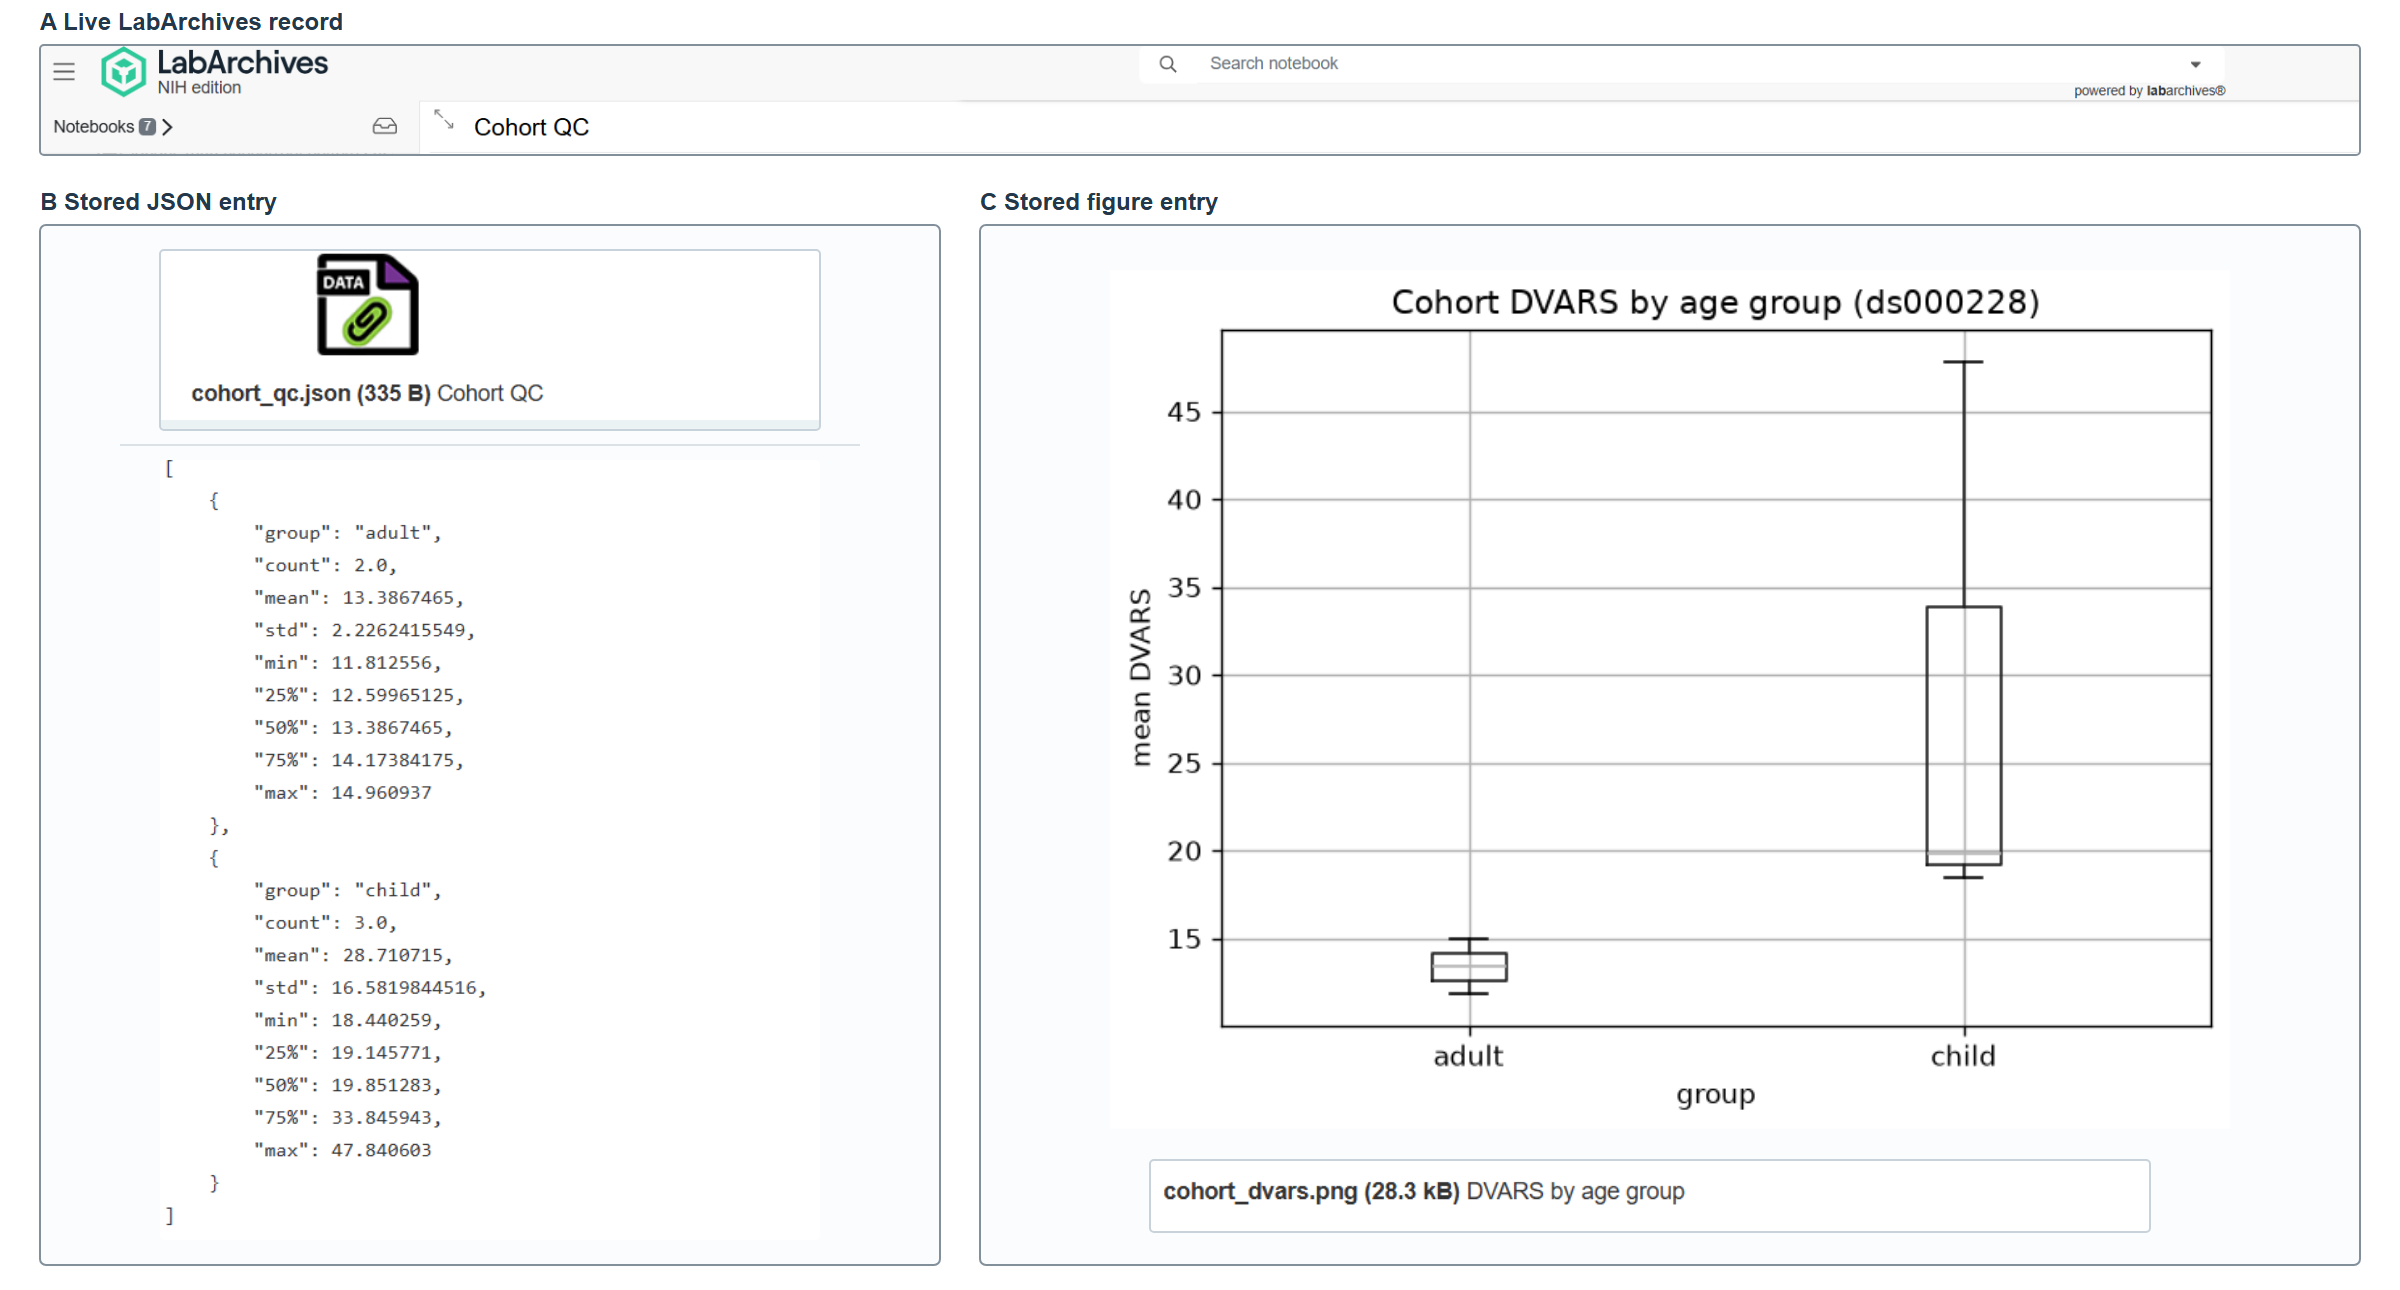
\includegraphics[width=\textwidth]{../figures/cohort-dashboard-example.png}
    \caption{The LabArchives page produced by the second stage, showing the
    cohort summary, its formatted preview and the uploaded figure.}
    \label{fig:dashboard}
\end{figure}

\section*{(2) Availability}
\vspace{0.5cm}

\section*{Operating system}

Platform-independent (pure Python). Continuous integration runs on Ubuntu
24.04. labapi is also used on Windows 11 and is expected to run on macOS,
but these platforms are not covered by automated tests.

\section*{Programming language}

Python 3.10 or later; tested on Python 3.10 to 3.14.

\section*{Additional system requirements}

Network access to a LabArchives API endpoint, and an API access key ID and
password issued by LabArchives through the user's institution. The optional
browser-based login requires a local installation of Chrome, Firefox or
Edge.

\section*{Dependencies}

cryptography ($\geq$ 50), lxml ($\geq$ 6.1.1), requests ($\geq$ 2.33) and
typing-extensions. Optional extras: \texttt{builtin-auth} adds selenium and
installed-browsers for browser-based login, and \texttt{dotenv} adds
python-dotenv for loading credentials from a \texttt{.env} file.

\section*{List of contributors}

Christoph Li (lead developer and maintainer); Josh Lawrimore (concept, code
and code review); Adam G. Thomas (code); Dustin Moraczewski (project
direction). Affiliations are given above.

\section*{Software location:}

{\bf Archive}

% TODO: replace the version, DOI and date if a 1.2.x patch release is cut
% for the submission.
\begin{description}[noitemsep,topsep=0pt]
	\item[Name:] Zenodo
	\item[Persistent identifier:] \url{https://doi.org/10.5281/zenodo.22021367}
	\item[Licence:] MIT
	\item[Publisher:] Christoph Li
	\item[Version published:] 1.2.0
	\item[Date published:] 20/08/2026
\end{description}

{\bf Code repository}

% TODO: confirm the date the repository was made public. GitHub reports the
% repository was created on 27/05/2025; codemeta.json gives 15/12/2025.
\begin{description}[noitemsep,topsep=0pt]
	\item[Name:] GitHub
	\item[Identifier:] \url{https://github.com/nimh-dsst/labapi}
	\item[Licence:] MIT
	\item[Date published:] 27/05/2025
\end{description}

Documentation: \url{https://nimh-dsst.github.io/labapi/}. Package:
\url{https://pypi.org/project/labapi/}.

\section*{Language}

English

\section*{(3) Reuse potential}

In the work described here, labapi writes pipeline outputs to the page that
documents an experiment, reads them back for a later analysis stage, and
backs up whole notebooks. Nothing in labapi is specific to neuroscience.

The Systems Neuroscience Imaging Resource, an NIMH core facility for imaging
and image analysis, backs up its notebooks with labapi, and the backup
feature was written together with that facility \citep{labapi_issue_264}.
Developers can build on the object model in the same way muronto and
save-my-jupyter do. The repository's examples are starting points for
common tasks: uploading CSV files as formatted tables and downloading them
again, keeping a folder of JSON files in sync with a page, downloading a
folder, and logging model runs.

Questions and bug reports go to the GitHub issue tracker, which has forms
for bug reports and feature requests. The contributing guide covers setting
up a development environment, running both test suites and opening a pull
request, and contributors can also write to the corresponding author. Each
release has its own documentation and is published on PyPI and archived on
Zenodo.

\section*{Acknowledgements}

The contributions of the NIH authors were made as part of their official
duties as NIH federal employees, are in compliance with agency policy
requirements, and are considered Works of the United States Government. The
findings and conclusions presented in this paper are those of the authors
and do not necessarily reflect the views of the NIH or the U.S. Department
of Health and Human Services (HHS). Mention of trade names, commercial
products or organisations does not imply endorsement by the U.S. Government.

% Ubiquity Press AI policy: use beyond copyediting must be declared. Placed in
% Acknowledgements, following GravDyn (JORS 2026). TODO: re-read the policy
% before submission.
Generative AI was used in developing the software and preparing this paper.
The authors designed labapi's foundational architecture and implemented its
core. AI tools subsequently assisted with development, testing, maintenance,
release work, documentation and manuscript preparation: they generated code,
contributed to tests, opened pull requests and issues, and drafted and
edited documentation and manuscript text. The authors reviewed and accepted
all AI-assisted software changes through public pull requests, reviewed and
revised all AI-assisted text, and take full responsibility for the software
and this paper. The tools used were Anthropic's Claude (Opus 4.6, Opus 4.8,
Opus 5, Sonnet 4.6, Sonnet 5 and Fable 5) and OpenAI's Codex (GPT-5.4,
GPT-5.5, and GPT-5.6 Luna, Sol and Terra), the latter accessed through the
HHS Enterprise agreement.

\section*{Funding statement}

This work was supported in part by the Intramural Research Program of the National
Institutes of Health, under National Institute of Mental Health project
ZICMH002960. This project has been funded in whole or in part with federal
funds from the National Cancer Institute, National Institutes of Health,
under Contract No.\ 75N91019D00024.

\section*{Competing interests}

% TODO: confirm with all authors.
The authors declare that they have no competing interests.

\bibliographystyle{unsrtnat}
\bibliography{../paper}

\vspace{2cm}

\rule{\textwidth}{1pt}

{ \bf Copyright Notice} \\
Authors who publish with this journal agree to the following terms: \\

Authors retain copyright and grant the journal right of first publication with the work simultaneously licensed under a \href{http://creativecommons.org/licenses/by/3.0/}{Creative Commons Attribution License} that allows others to share the work with an acknowledgement of the work's authorship and initial publication in this journal. \\

Authors are able to enter into separate, additional contractual arrangements for the non-exclusive distribution of the journal's published version of the work (e.g., post it to an institutional repository or publish it in a book), with an acknowledgement of its initial publication in this journal. \\

By submitting this paper you agree to the terms of this Copyright Notice, which will apply to this submission if and when it is published by this journal.

\end{document}
